\section{Discusión}

La materialización del Portal Agro-Comercial del Huila y su posterior análisis arquitectónico nos sitúan frente a una encrucijada paradigmática que trasciende los límites de la ingeniería de software convencional. La experiencia de campo acumulada en el municipio de Teruel ha revelado una verdad incómoda para la academia: la brecha digital en el sector rural no es una herida que se cierre simplemente entregando un aplicativo funcional bajo la premisa de ``entregar y olvidar''. Por el contrario, dicha brecha solo se mitiga garantizando que la herramienta posea la resiliencia sistémica necesaria para sobrevivir a la evolución del mercado, a la rotación de personal técnico y a la obsolescencia tecnológica.

En el contexto del desarrollo de software para el agro, donde los proyectos a menudo mueren por falta de mantenimiento evolutivo (``Software Rot''), no basta con escribir código limpio (\textit{Clean Code}); es imperativo diseñar sistemas vivos. En esta sección se analizan las tensiones identificadas durante el estudio, interpretando los resultados bajo la óptica teórica de los \textit{Feature Toggles} y contrastando la realidad local del SENA con la literatura global de ingeniería de software.

\subsection{El Dilema Ético-Técnico: Carga Cognitiva vs. Resiliencia Operativa}

Nuestra propuesta arquitectónica plantea un compromiso de ingeniería (\textit{trade-off}) que no puede ni debe ocultarse: la introducción deliberada de lógica condicional en el flujo de control. Bajo paradigmas tradicionales de desarrollo, el código del Portal sería lineal, secuencial y predecible; con la inyección de la arquitectura de toggles, se transforma en un árbol de decisiones ramificado y dinámico.

Autores como \cite{sharma2024complexity} advierten, respaldados por datos empíricos de la industria, que esta práctica incrementa significativamente la carga cognitiva del desarrollador. Leer, depurar y razonar sobre un código con múltiples puntos de bifurcación es objetivamente más complejo que analizar un script lineal. Ante esto, surge la pregunta obligada de investigación: ¿Se justifica incurrir en esta sobrecarga de ingeniería para un proyecto de alcance local y recursos limitados?

Nuestra postura es afirmativa y categórica. En el ecosistema digital rural, la \textbf{confianza del usuario} es un activo extremadamente volátil. Si un agricultor, que quizás está venciendo años de resistencia cultural a la tecnología, intenta acceder a la plataforma tras una actualización y encuentra un error crítico o una pantalla en blanco, es altamente probable que abandone la herramienta de forma definitiva. En este escenario, la estabilidad operativa no es simplemente un requisito no funcional; es la base fundamental de la propuesta de valor.

Al adoptar los toggles, estamos efectivamente intercambiando complejidad de desarrollo (que asume el ingeniero) por seguridad operativa (que beneficia al campesino). Esta inversión se alinea con la visión de \cite{rahman2016msr}: el objetivo final es desmitificar el proceso de despliegue. Buscamos que una actualización deje de ser un evento traumático para convertirse en una tarea rutinaria. Para un equipo pequeño como el nuestro, que carece de capacidad para sostener mesas de ayuda 24/7, la posibilidad de desactivar una funcionalidad defectuosa en segundos (\textit{Kill Switch}) no tiene sustituto técnico viable.

\subsection{El Desafío de la Deuda Técnica y la Psicología del Desarrollador}

Ignorar los riesgos de sostenibilidad a largo plazo sería intelectualmente irresponsable. Un hallazgo crítico de nuestra fase de investigación es que el mayor enemigo de los \textit{Feature Toggles} no es el compilador ni el rendimiento, sino la psicología humana.

La literatura es contundente al respecto: los toggles mal gestionados son una de las fuentes más agresivas de deuda técnica. Investigaciones como las de \cite{ortiz2021toggledebt} y \cite{abdalkareem2021removal} documentan un patrón de comportamiento peligroso: la inercia del desarrollador. Existe una tendencia natural a asumir que eliminar una bandera estable implica un riesgo innecesario (``Si funciona, no lo toques''), lo que lleva a que toggles diseñados para durar dos semanas permanezcan en el código base durante años, creando capas geológicas de lógica obsoleta.

Si nuestra propuesta se implementa sin una disciplina férrea, el Portal Agro-Comercial corre el riesgo de convertirse en un sistema ``zombi'', saturado de rutas de código muerto. Para mitigar este problema, adoptamos la postura radical sugerida por \cite{sridharan2020piranha} con la herramienta Piranha: la limpieza debe ser obligatoria y, preferiblemente, automatizada. Proponemos que la \textit{Definición de Hecho} (DoD) en Scrum incluya explícitamente la eliminación del toggle. El éxito del proyecto depende de interiorizar culturalmente que \textbf{borrar código viejo} es una actividad tan productiva y vital como escribir código nuevo.

\begin{figure}[htbp]
    \centering
    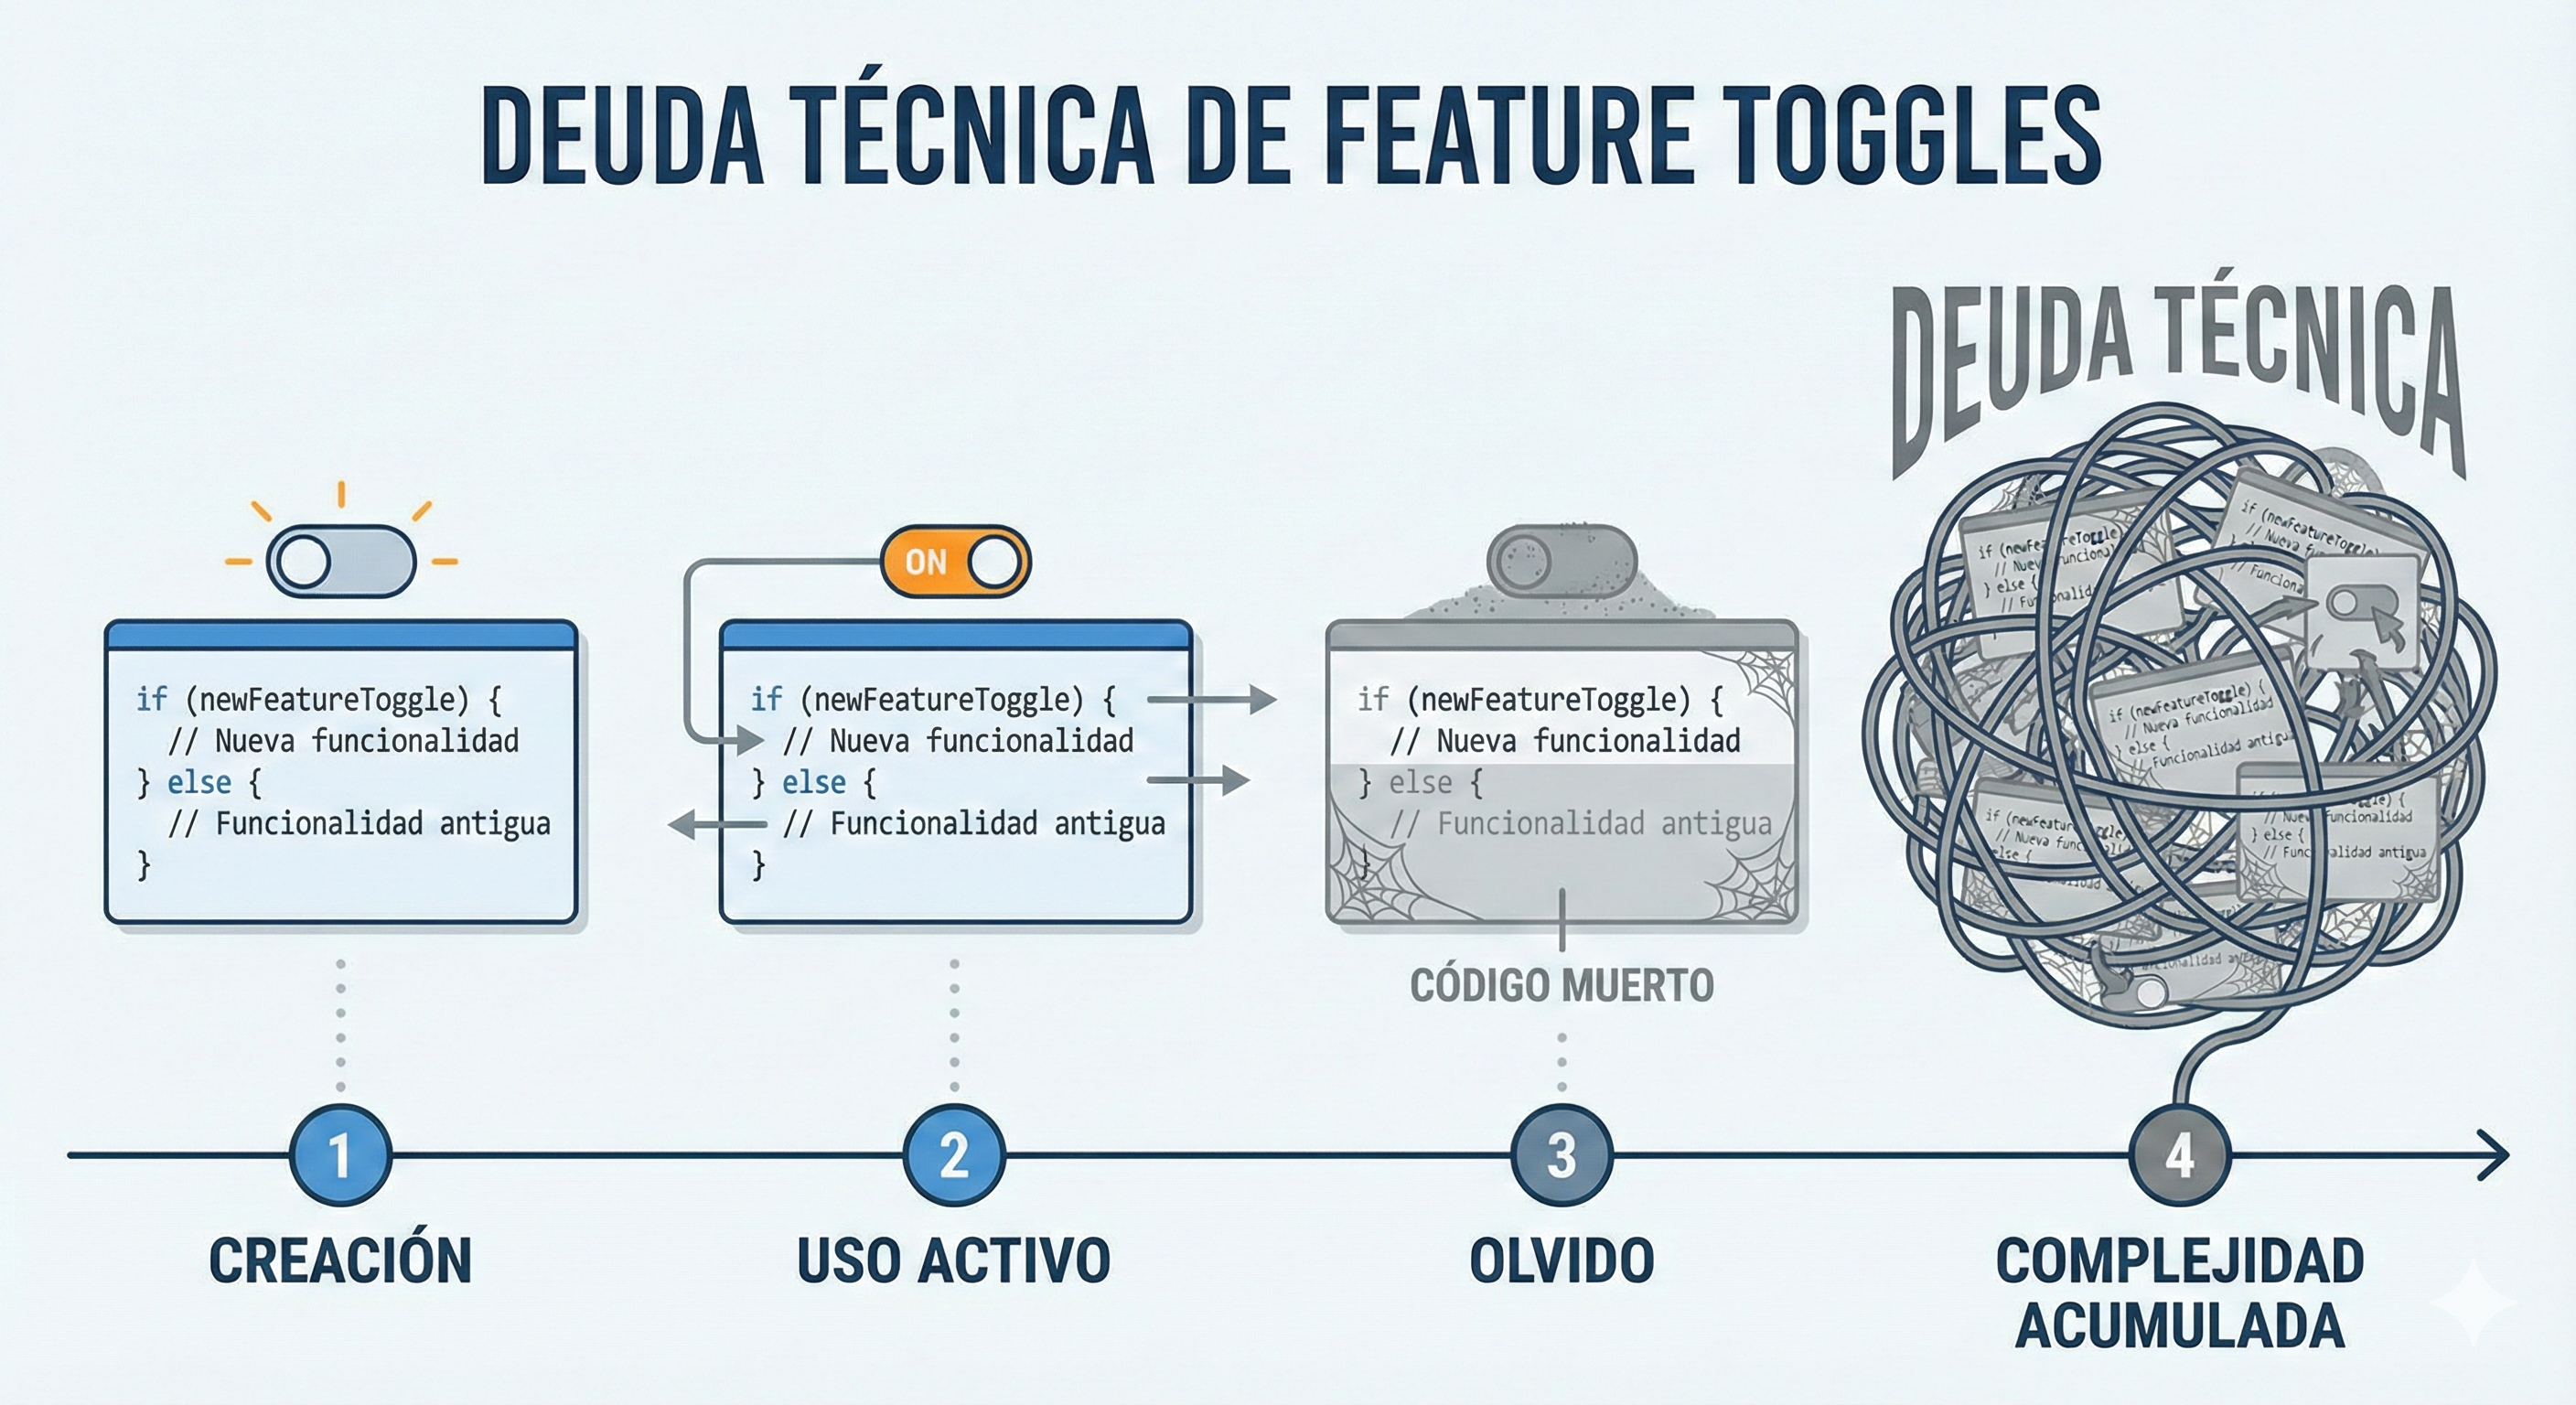
\includegraphics[width=0.9\columnwidth]{graphics/deuda_toggles.png}
    \caption{Representación del ciclo de vida de un Feature Toggle y el riesgo acumulativo de la deuda técnica. Un toggle no eliminado se convierte en ``código muerto'', aumentando exponencialmente la entropía del sistema.}
    \label{fig:deuda_toggles}
\end{figure}

\subsection{La Explosión Combinatoria y el ``Infierno de la Configuración''}

Un aspecto que superó nuestras expectativas iniciales de complejidad fue la gestión de las interacciones entre banderas. Al escalar el diseño teórico, se evidenció el problema descrito por \cite{smith2022interdependencies} en el ecosistema de Microsoft Office: los toggles no existen en el vacío; interactúan entre sí.

Considérese el siguiente escenario: activar el toggle \texttt{Pago\_En\_Linea} mientras se mantiene desactivado el toggle \texttt{Calculo\_Impuestos}. Esto podría generar un estado inconsistente de negocio donde se procesan transacciones sin retenciones fiscales, exponiendo a la plataforma a riesgos legales. Este fenómeno, denominado por \cite{hal2022interaction} como ``Interacción de Features'', representa el mayor riesgo lógico de la arquitectura propuesta. Si tenemos $N$ toggles activos, el sistema tiene teóricamente $2^N$ estados posibles, una cifra que crece exponencialmente y hace imposible el aseguramiento de calidad manual.

Para mitigar este riesgo, el sistema no puede depender de la memoria del desarrollador. Es imperativo implementar matrices de compatibilidad automatizadas en el pipeline de CI/CD que validen no solo que el código compile, sino que la combinación activa de banderas sea semánticamente consistente. Esto eleva el nivel de exigencia técnica para los futuros mantenedores del proyecto, requiriendo pruebas de integración más sofisticadas.

\subsection{Vectores de Seguridad y Feature Leaking}

Se identificó un vector de riesgo frecuentemente subestimado en implementaciones académicas: la seguridad de la configuración. Tal como advierten \cite{li2020capture} y muy recientemente \cite{wang2025tsdetector}, exponer la lógica de los toggles en el cliente (Frontend) conlleva riesgos críticos de seguridad.

Si el servidor envía al navegador un objeto JSON detallado con todas las banderas (ej. \texttt{\{"AdminPanel": false, "DiscountV2": true\}}), se abre la puerta a que un usuario malintencionado con conocimientos técnicos básicos manipule la configuración local para habilitar funciones restringidas o experimentales. Este fenómeno, denominado \textit{Feature Leaking}, compromete la integridad del negocio.

La arquitectura debe ser ``paranoica por diseño'': el servidor .NET nunca debe enviar al cliente configuraciones que impliquen decisiones lógicas sensibles o de seguridad. El cliente solo debe recibir el resultado final de la evaluación para propósitos de renderizado, nunca las reglas completas ni el estado de funcionalidades administrativas ocultas.

\subsection{Rompiendo el Mito del ``Software Rural Simple''}

Finalmente, este trabajo busca desafiar el prejuicio arraigado de que el software dirigido al sector agropecuario debe ser tecnológicamente básico o simplista. Este enfoque es conceptualmente erróneo y condescendiente.

Como sostienen \cite{garcia2007informacion}, las organizaciones complejas —y una red de productores agrícolas lo es— requieren sistemas avanzados de gestión del conocimiento. El software rural, precisamente por operar en entornos adversos de conectividad, soporte y alfabetización, demanda arquitecturas tan robustas y resilientes como las del sector financiero o de telecomunicaciones. La capacidad de activar y desactivar módulos granulares sin afectar la operación global demuestra que es posible y necesario llevar ingeniería de alto nivel a proyectos de impacto social. Se trata de innovar en la arquitectura oculta para proteger y simplificar la experiencia visible del usuario final.
